\chapter{Implementation} \label{implementation}


%5\section{Extension Structure}

As explained in \ref{browserExtensions}, the extension is split into different files for both security reasons and other separation of concerns.
Figure \ref{fig:project_structure} puts into more detail the exact structure of the extension in context with some of the real files being used.


\begin{figure}[h]
	\centering
	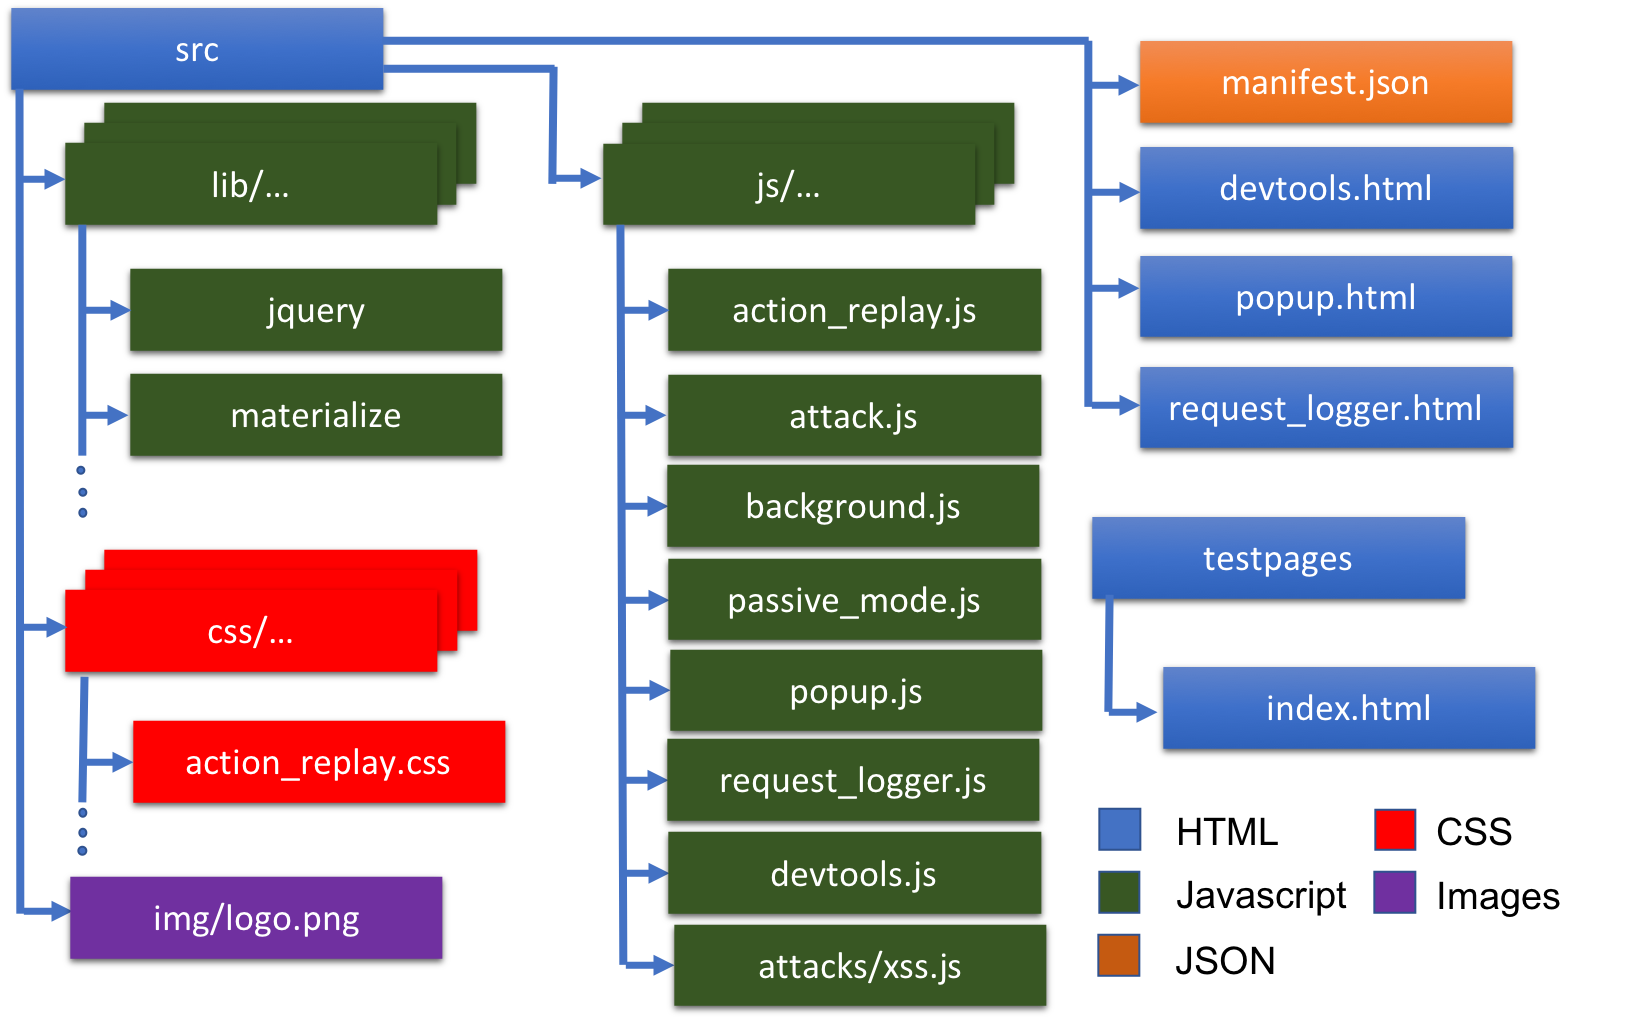
\includegraphics[width=0.9\textwidth]{images/project_structure.png}
	\caption{The directory structure used for the project}
	\label{fig:project_structure}
\end{figure}

We have arranged the files in question into 2 separate subfolders - the \texttt{testpages} directory keeps the source code for the test harness page with vulnerabilities, while the \texttt{src} directory keeps all the other extension related code. \\

Within \texttt{src} we find different folders for separate concerns - \texttt{lib} stores any library code we have imported from a third-party, \texttt{css} keeps custom styles used across the extension, \texttt{img} is where any images are kept, \texttt{js} holds any custom produced Javascript files, and is where most of the logic within the extension lives. \texttt{src} also contains the \textit{manifest} file, and any HTML page code. 

\section{Manifest}

The manifest is where the extension declares its intentions by enumerating all the scripts and files to be accessed, as well as the permissions required to run the extension as an add-on to the browser. This file is necessary due to security reasons; each extension is expected to run as a standalone program within the browser. Any dependencies are to be declared and included within the package before the program is run, with the exception of contents that are whitelisted in the declared \textit{Content Security Policy} (CSP) directive within the file. We are using the recommended default CSP directive of \texttt{script-src 'self'; object-src 'self'}. This policy actively prevents notoriously dangerous Javascript functions from being evaluated, disables in-line Javascript functionality (which enforces a separation of content from behaviour), and, as the name suggests, will only load scripts and files locally available to the package \cite{chromeExtensionCSP}. \\ 

A potential methodology to use in a setting like this would be to employ a bundler to create a single minified (or compressed) \texttt{.js} file that includes all the required libraries and code to be imported. An example of this is  \textit{Webpack} \footnote{\url{https://webpack.js.org/}} - we did not employ a bundler like this as we learned about its uses later into the project. Furthermore, we are including a relatively small number of third-party sourced code, making this a small practical concern. \\

Other noteworthy details from the manifest file include:

\begin{itemize}
	\item The \texttt{devtools\_page} directive - this is necessary to access the developer tools API's within the extension, which provide extra information when using the extension such as the contents of the requests sent at any given time. See \ref{devtools}.
	
	\item The \texttt{web\_accessible\_resources} directive allows us to specify resources which should be accessible in the context of a normal browsing experience. This is a feature enabled in the more recent 2.0 version of the manifest, which blocks resources by default unless they are whitelisted in this manner. This prevents malicious attacks on the extension, such as fingerprinting or exploiting XSS vulnerabilities \cite{chromeExtensionWebAccessibleResources}. An example of a resource included here is the \texttt{request\_logger.html} page.
	
	\item The \texttt{content\_scripts} to be included in every page are also defined here - this includes both CSS files as well as third-party libraries and Javascript vulnerability scanning files.
\end{itemize}

\section{Test harness}

In order to be able to appropriately test for features in development for this extension it is necessary to have access to a fragile website. It would not be ethical to use a website in production to test Gentoo against; doing so could result in all manner of adversities for the owner of that web address. That is under the assumption that we could firstly find a fragile website to test against; despite the prevalence of security weaknesses spread through the web, it is inherently a difficult task to identify and exploit these. Therefore, we have developed a deliberately weak website to test against. As will be demonstrated in each of the following sections, this harness website (stored under \texttt{testpages/index.html}) can be used to showcase an example of each vulnerability and consequent attack. \\

In order to emulate the website as a server, we are using the out-of-the-box implementation of Python's \texttt{SimpleHTTPServer}. To run this, we simply have to run \texttt{python3 -m http.server 8000} to start a server on the localhost at port 8000. This allows us to submit forms and thus emulate query parameter submissions.

\section{Popup page}

This is the main interaction point for a user utilizing the extension. The layout of this page makes a clear distinction between the different features available to use in the extension. \\

\begin{figure}[h!]
	\centering
	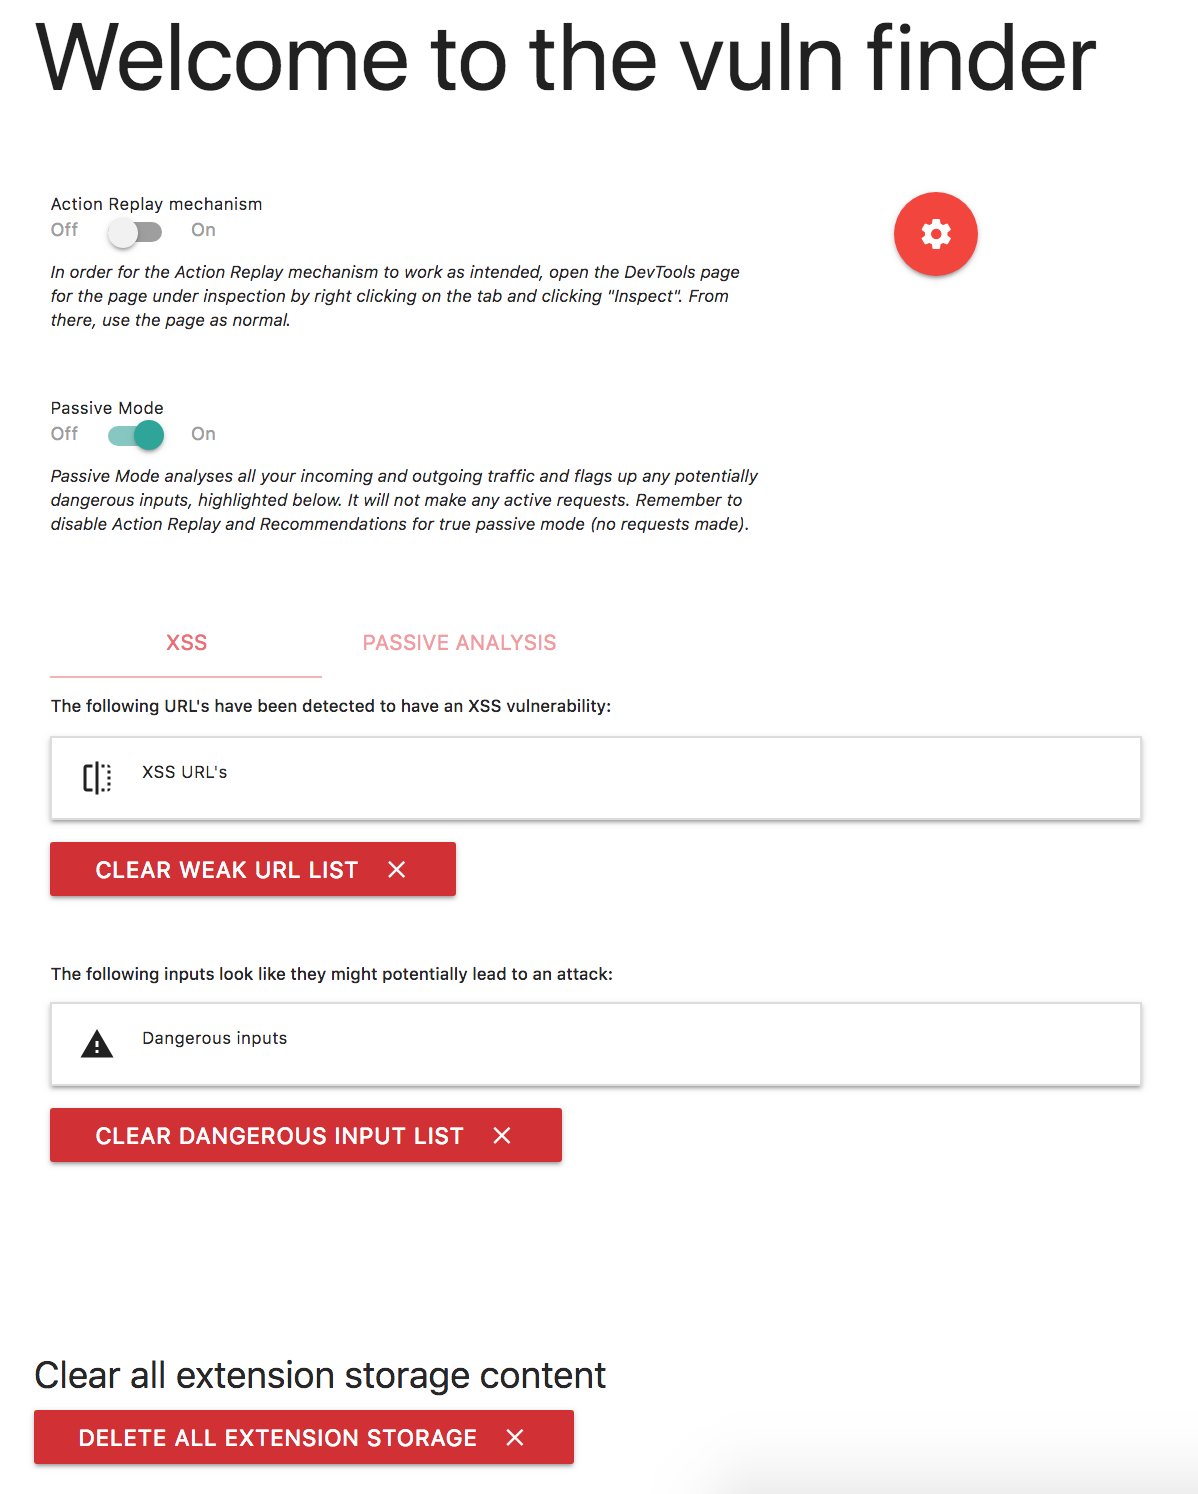
\includegraphics[width=0.8\textwidth]{images/popup_full.png}
	\caption{The main contents of the popup page when first clicked by a user}
	\label{fig:popup_full}
\end{figure}

This page offers an accessible means for tweaking and toggling all the options available in the extension, as well as viewing and analysing the outputs from the different modes of running the extension.  


\section{Background Page}

The background page we are using in the extension is a persistent page, meaning it is constantly running. This is in contrast to event background pages, which are opened and closed as necessary depending on the occasion. We are using this page to listen for messages sent from other scripts to be able to set aesthetic updates, as well as establishing a connection with the \texttt{devtools} page to subscribe to and forward custom request messages to content scripts.

\section{Request Logger}

This page is designed to capture information from attacks that have successfully hijacked Javascript execution and diverted a user to this page. This functionality is paramount in being able to detect XSS vulnerabilities in Gentoo. In order to be accessible from any other window, it must be declared as a \texttt{web\_accessible\_resource}. It captures the page it was referred from and reports it as a page where a vulnerability exists.

\section{Devtools} \label{devtools}

The devtools page has access to a specific set of API's designed to extend the experience for web developers using the browser. This includes access to the currently inspected window, the developer panels, and network request information \cite{chromeExtensionDevTools}. \\

\begin{figure}[h]
	\centering
	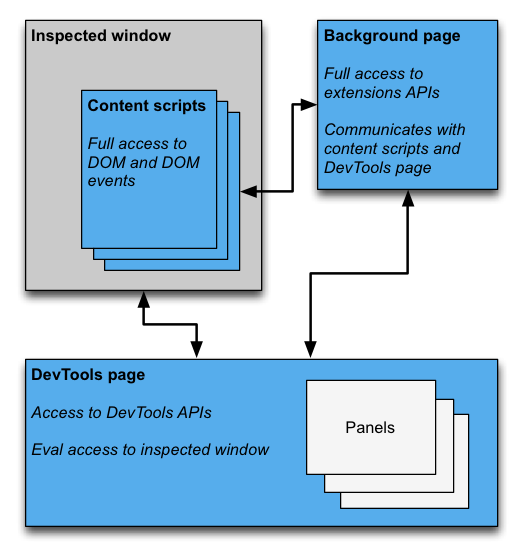
\includegraphics[width=0.55\textwidth]{images/devtools-extension.png}
	\caption{An extension making use of the DevTools API's further extends the capabilities of a standard Chrome Extension. Diagram from \cite{chromeExtensionDevTools}.}
	\label{fig:devtools_extension}
\end{figure}

More specifically, we are interested in the \texttt{devtools.network} API - this provides access to every request once it has finished. This contains a wealth of information which is otherwise difficult to obtain without using the devtools API. One of the APIs we are also using in the extension is the \texttt{chrome.webRequest}. This gives us access to several different events at different points of the lifetime of the request. It allows us to access some headers as well as change a limited set of these. It however does not provide sufficient information for the purposes of the extension - \texttt{devtools.network} gives access to the response content of any given request, which is vital in analysing outputs from a request to create attack correlations. Accessing the \texttt{devtools} APIs requires the Developer tools to be open for the page in question, which is only a small inconvenience when using the extension.

\section{Message Design}

To better understand the structure of the extension and how each feature ahead is to be implemented, it's good to create a high level overview of messaging between each component.  \\

\begin{figure}[h]
	\centering
	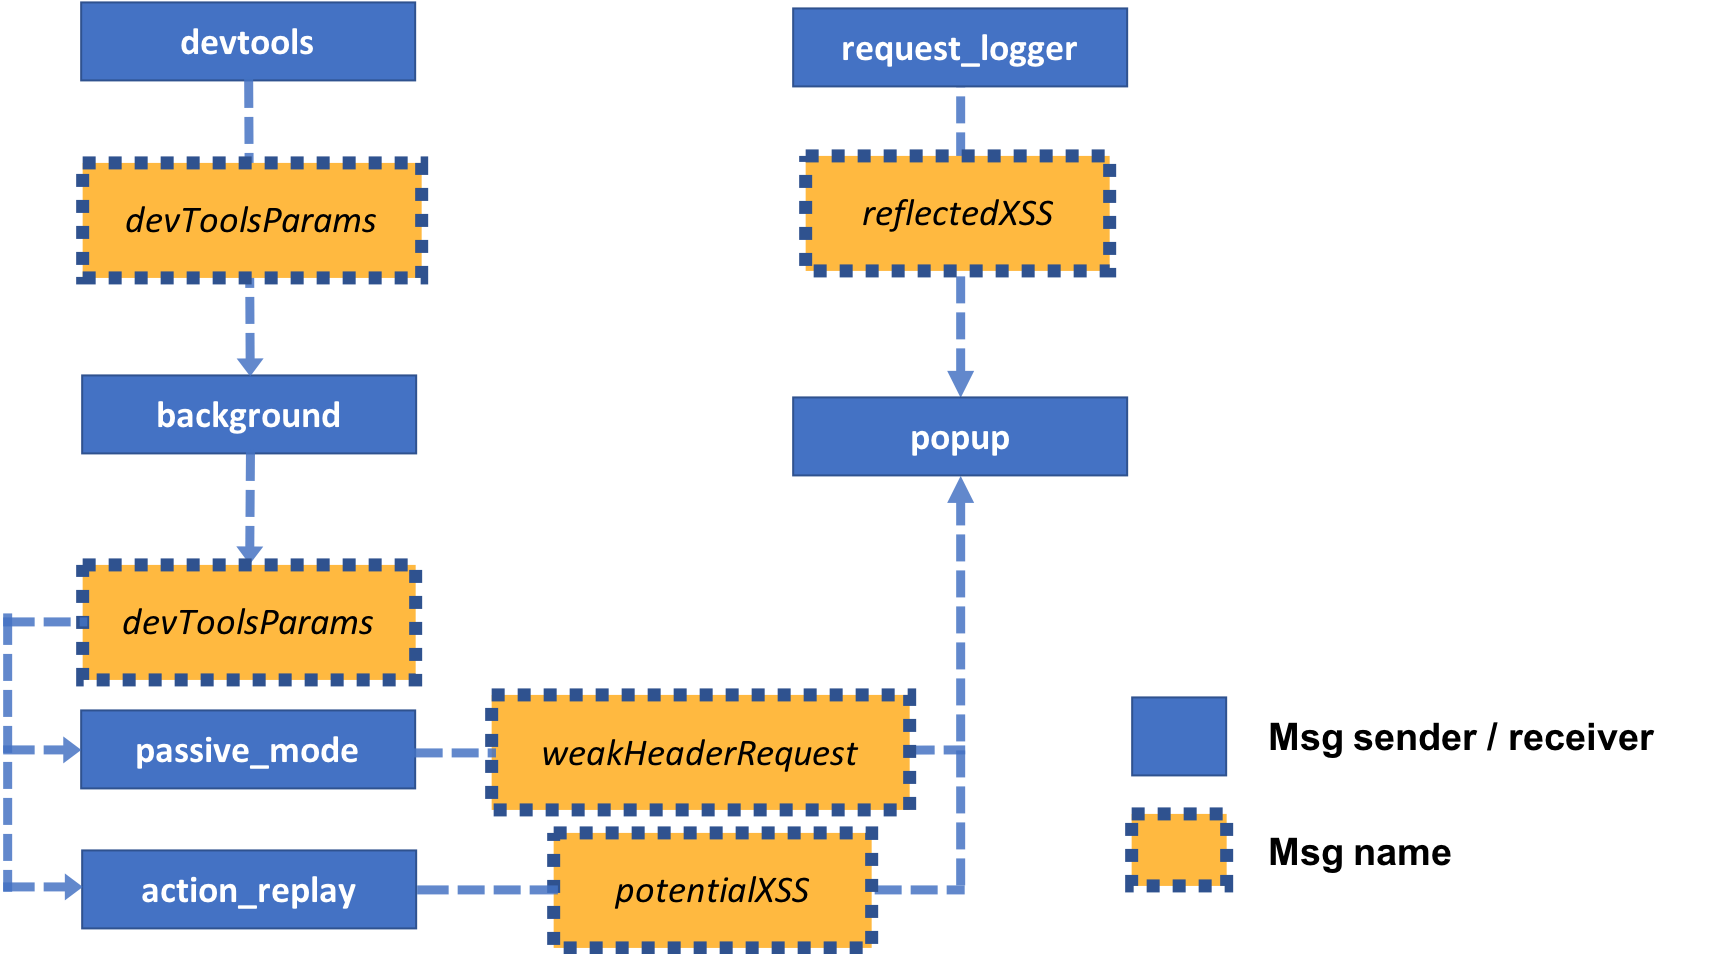
\includegraphics[width=0.95\textwidth]{images/message_passing.png}
	\caption{This diagram illustrates the passing of messages within the different components in the extension}
	\label{fig:message_passing}
\end{figure}

In order to analyse the requests being made in different context scripts, the \texttt{devtools} script gathers every request made in the page which has the Developer Tools inspection windows open. Since this page cannot directly pass messages to the content scripts \cite{chromeExtensionDevTools}, it uses the background page as a mediator. It establishes a connection to the background page and passes to it every request it picks up. The background page then forwards these messages to the different content scripts that analyse the requests - \texttt{action\_replay} and \texttt{passive\_mode}. \\

Whenever a request causes the \texttt{request\_logger} page to be loaded, the page captures the information from the page it has just been referred to from, and forwards this information in a message to the \texttt{popup} page to update the list of vulnerable URLs. To toggle the enabling or disabling of the Action Replay algorithm, the popup page sends a message to the \texttt{action\_replay} script each time the corresponding switch is clicked. When the Action Replay is mid analysis, it will produce a warning list of inputs it has considered to be potentially dangerous, and passes a message to the \texttt{popup} page when it has detected this. Similarly, in the \texttt{passive\_mode} script, a message is passed to the \texttt{popup} alerting to any suspicious request behaviour. The \texttt{background} script also listens to several of these messages, and consequently updates the UI badge aesthetics, alerting the user to fresh information to analyse in the extension.

\section{Chrome Storage} \label{storageSpecs}

Google offers access to the \texttt{chrome.storage} API, which is a specialised storage designed for the needs and uses of an extension. This is an asynchronous storage that allows storing of objects (not solely strings as is found in \texttt{localStorage}). Perhaps most practically, it also allows each content script to access storage data without the need to relay this information through the background page. At the start of the project we were using \texttt{localStorage}, but quickly switched to \texttt{chrome.storage} once we ran into the hassles of using this (converting to and from a \textit{string} type on access and storage, as well as using the \texttt{background} as a proxy for every access). \\

We are using this storage to keep a variety of settings and flags, as well as different lists of requests and analysis. Namely: 

\begin{itemize}
	\item \texttt{passiveModeRequests} - This collects all the requests gathered when running the Passive Mode in the extension. This stores request and response params, headers and cookies, as well as the response content and the URL pertinent to the request.
	
	\item \texttt{passiveModeWeakHeaderRequests} - Initially intended to store the requests which have been detected to have weak security Headers, this stores an array of requests with properties similar to the \texttt{passiveModeRequests}. The difference between what is stored is that in this array we also store a list of warnings added to the request by the passive mode if it has found any worrying information during its scan.
	
	\item \texttt{settings} - This is an array of flag settings determined in the settings section of the extension. It stores information such as the \texttt{recommenderSensitivity}, \texttt{passiveModeCSRFEnabled} and \texttt{passiveModeWindowSize}.
	
	\item \texttt{cachedSettings} - This stores the same information as \texttt{settings}; \texttt{cachedSettings} are used to store settings before these are saved in the settings window.
	
	\item \texttt{potentialXSS} - This stores a list of user controlled inputs involved in XSS detection. Each input stores its type - \textbf{cookie}, query \textbf{param}eter or \textbf{header}. The input also stores the URL of origin, and the name and corresponding value of each value in consideration.
	
	\item \texttt{ARrequests} - This list stores every request that is captured within the currently / last recorded session of the Action Replay algorithm. The information kept per request is similar to that kept in \texttt{passiveModeRequests}.
	
	\item \texttt{ARSession} - This flag keeps track of whether the current Action Replay session is recording or stopped.
	
	\item \texttt{enableAR} - Enables or disables Action Replay in the current page.
	
	\item \texttt{enablePassiveMode} - Enables or disables Passive Mode in the current page.
	
\end{itemize}

\section{Recommendations} \label{recommendations}

One of the large features intended for implementation in this project was the use of suggestions whilst browsing a page to attempt vulnerability exploits. This provides a low-effort means for a penetration tester to quickly test different types of attacks on a webpage. \\

The recommendations in the extension work by analysing the contents of the page, and tweaking the page accordingly. It begins by reviewing every \texttt{form} tag in the page - for each form found in the page, it will detect any child \texttt{input} tags, and for the first of these will create a sibling node which acts as a prompt to analyse the page further. \\

The sibling node with the text \textit{Investigate form} is made into a clickable element, and upon click will initiate an attack attempt against the input in question. 

\begin{figure}[h]
	\centering
	\begin{subfigure}{.5\textwidth}
		\centering
		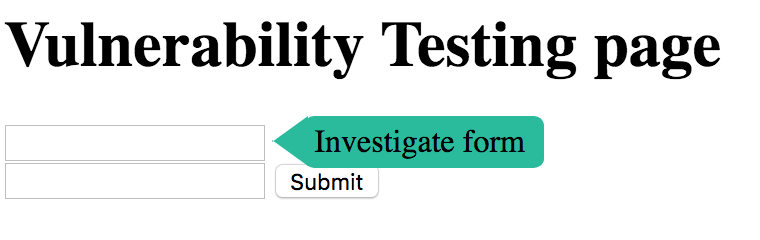
\includegraphics[width=.8\linewidth]{images/test_page_investigate_form.png}
		\label{fig:test_page_investigate_form}
	\end{subfigure}%
	\begin{subfigure}{.5\textwidth}
		\centering
		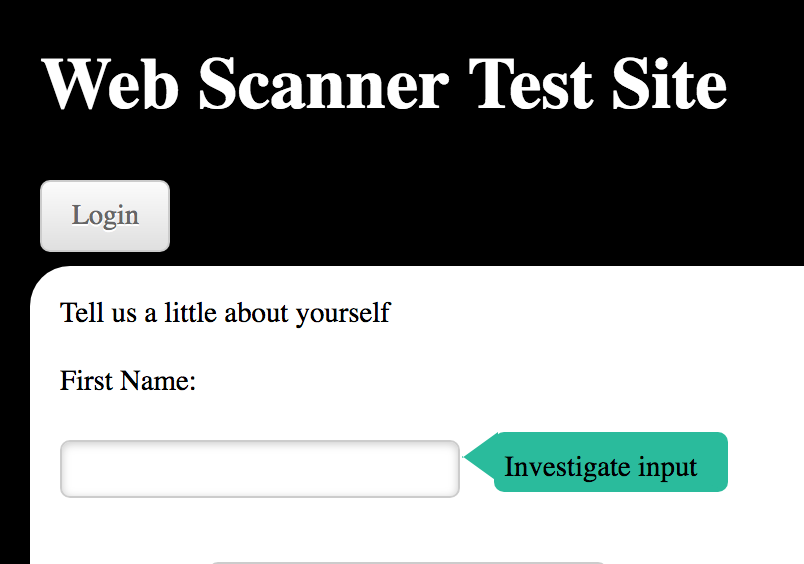
\includegraphics[width=.8\linewidth]{images/web_scanner_investigate_form.png}
		\label{fig:whiteBox}
	\end{subfigure}
	\caption{The \textit{Investigate Form} input being added to different pages allows a user to attempt attacks against the page in question.}
	\label{fig:investigate_form}
\end{figure} 

\subsection{Recommendation Sensitivity}

With the above implementation it would not be possible to ascertain whether an input that wasn't first in a form was susceptible to vulnerabilities or not. Adding the \textit{Investigate Form} button to every input in a page will \textit{usually} create too much clutter and make the page harder to use. It also creates elements for hidden inputs, which is likely to shift the contents of the page in unexpected ways. \\

As a result, we added a setting to tweak the sensitivity of the Recommendations - the default setting of \textbf{1} will apply the algorithm above, adding a button for the first \texttt{input} tag per \texttt{form} on a page. Setting it to \textbf{2} will now add the button as above for \textbf{every} \texttt{input} tag per \texttt{form} on a page. The highest sensitivity (\textbf{3}) will append this button for every input in a page, regardless of being within a \texttt{form} tag or not. \\

\begin{figure}[h]
	\centering
	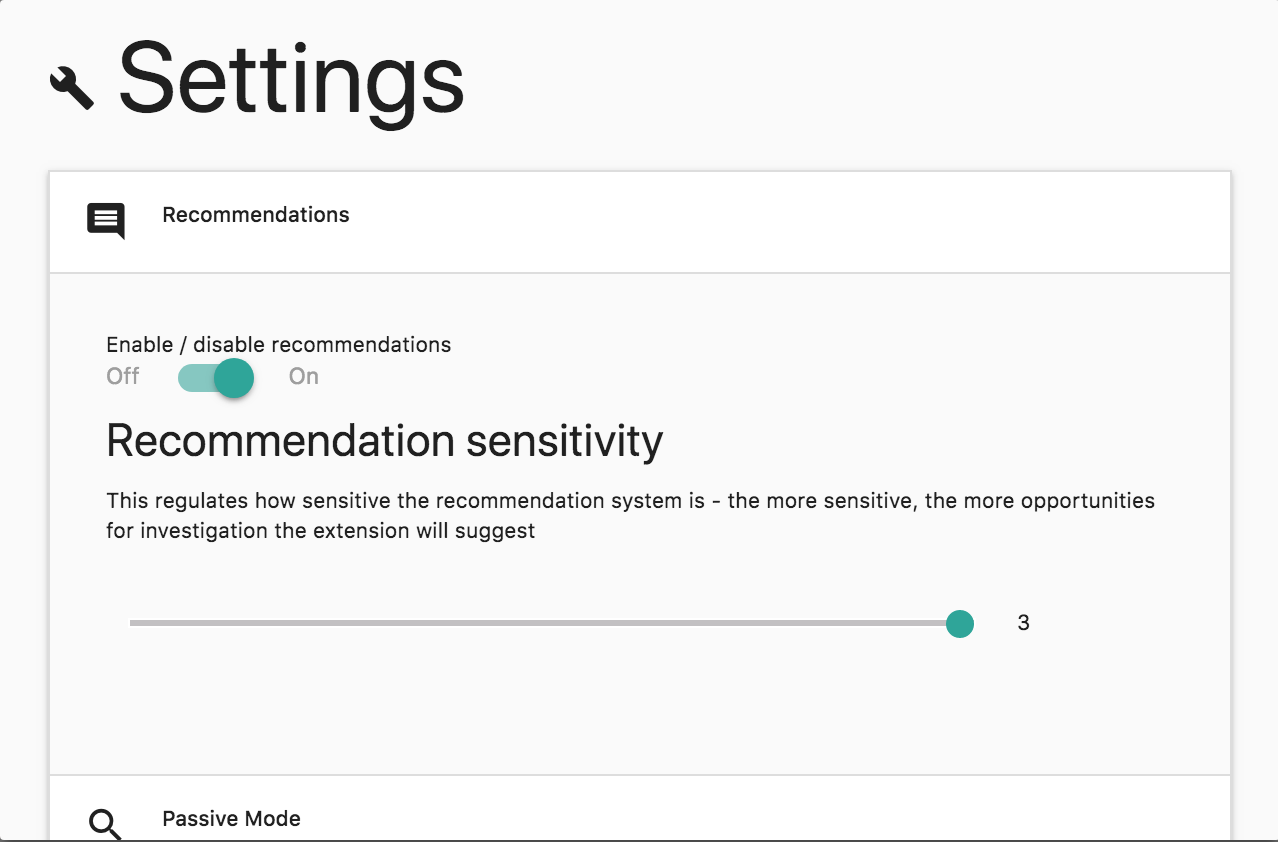
\includegraphics[width=0.7\textwidth]{images/tweaking_recommender_sensitivity.png}
	\caption{Changing the recommendation sensitivity within the settings tab}
	\label{fig:tweaking_recommender_sensitivity}
\end{figure}

This adds a bit more complexity to the method in question - the conventional Javascript and JQuery \texttt{submit()} methods work on form elements only. In order to submit the attack attempt for this sensitivity, we manually submit a request to the base URL of the current window, setting the query parameter with the name corresponding to the name of the input being selected. The value for this query parameter is the attack string with some modifications for correct URL encoding. These are:

\begin{enumerate}
	\item Replace the escaped character \texttt{\%20} with \texttt{+}. URL encoding rules state that for query parameters, a whitespace should be set to the \texttt{+} symbol instead
	
	\item Replace instances of the character \texttt{\&} with its URL encoded equivalent \texttt{\%26} - We are now within the specific value of the query parameter, so the \texttt{\&} character must be encoded, otherwise it would be mistaken for the start of another query parameter value within the overall URL, which breaks the attack.
\end{enumerate} 

\section{Action Replay} \label{actionReplay}

Action Replay is a another attack algorithm that works in a slightly different way. This mode allows a user to use the application as normal, with the expectation that the user narrows down the attack surface to a specific set (or sequence) of inputs. \\

Once the Action Replay mode is enabled, the extension adds a small input button to each page's body to allow the user to begin or terminate a session. A session is split into 2 parts - the recording phase and the replay phase. Once a session begins, it must firstly record the requests and inputs being made by the user. The extension does so by storing requests at the aforementioned array \texttt{ARrequests}. Once the user is happy that they have captured enough of the minimum behaviour required to potentially trigger a vulnerability, they can click the button once again to stop recording the session, thus starting the analysis and replay phase of the algorithm. At this stage the algorithm iterates through each of the requests stored in the \texttt{ARrequests} array and appends all of the captured user-controlled inputs to a list of custom \texttt{userInput}s to analyse. A meaningful user-controlled input in this case is either a \textbf{cookie}, a query \textbf{param}eter or a \textbf{header}. The \texttt{userInput} type has the parameters as defined for the data structure \texttt{potentialXSS} (see \ref{storageSpecs}). \\

\begin{figure}[h]
	\centering
	\begin{subfigure}{.5\textwidth}
		\centering
		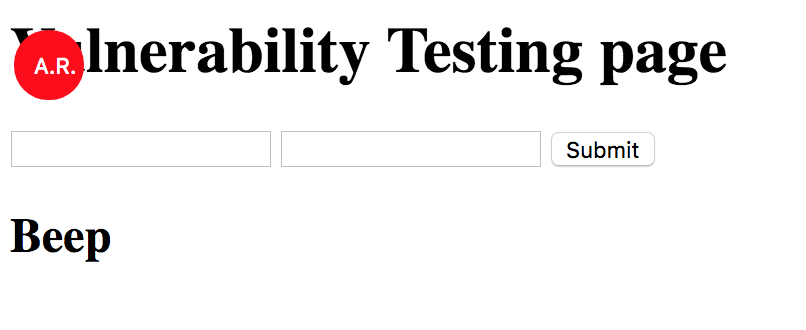
\includegraphics[width=.8\linewidth]{images/ar_initial.png}
		\label{fig:ar_initial}
	\end{subfigure}%
	\begin{subfigure}{.5\textwidth}
		\centering
		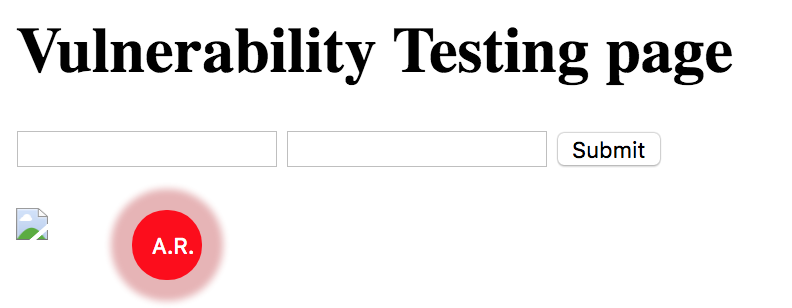
\includegraphics[width=.8\linewidth]{images/ar_recording.png}
		\label{fig:ar_recording}
	\end{subfigure}
	\caption{The Action Replay button before and during a session recording. A recording session starts and stops at the click of this button. In the interest of usability, the button can be moved by the user anywhere on the page so as to not obstruct other content indefinitely.}
	\label{fig:ar_stages}
\end{figure} 

In the interest of demonstrating a minimum behaviour within the time frame of the project, we analyse only the responses with the \texttt{Content-type} header set to \texttt{text/html}. This is because vulnerabilities in HTML responses are more readily detectable and easier to analyse than others (e.g. those in CSS files). \\

Once the algorithm has gathered this information, it filters out a series of user inputs it does not deem to be harmful through some heuristics. We focussed on detecting Cross Site Scripting (XSS) vulnerabilities, so the heuristics aim to detect any use of angled brackets (URL encoded or not) alongside potentially executable HTML tag names (such as \texttt{iframe}s, \texttt{img} tags or \texttt{script}). If a \texttt{userInput} is deemed to be potentially dangerous, we store these in the \texttt{potentialXSS} array and send a message to the extension warning of a detected reflection in the outputs. \\

After this intermediary warning, assuming some potentially dangerous user-controlled inputs were found, the algorithm begins to replay the requests, attempting different attacks from a stored suite. For each of the potentially dangerous inputs found earlier, it will apply each of the attacks. To do this, similarly to the process described at \ref{recommendations}, a new window is open, setting the user input to the specific attack value to test whether the attack worked on not. Accordingly, each attack is self-contained, so if it triggers a vulnerability (and Javascript was executed for example), it will (by design) refer itself to the \texttt{request\_logger}, which logs the vulnerability as described before.


\section{Passive Mode}

Passive Mode is designed to run in the background while browsing, gathering data about websites being visited and analysing requests to highlight warning signs of different vulnerabilities. It does so without making any requests of its own, meaning any potential misuse of a web application is entirely dependent on how the user navigates and uses it - this mode simply highlights information the user already has open access to. \\

\begin{figure}[h]
	\centering
	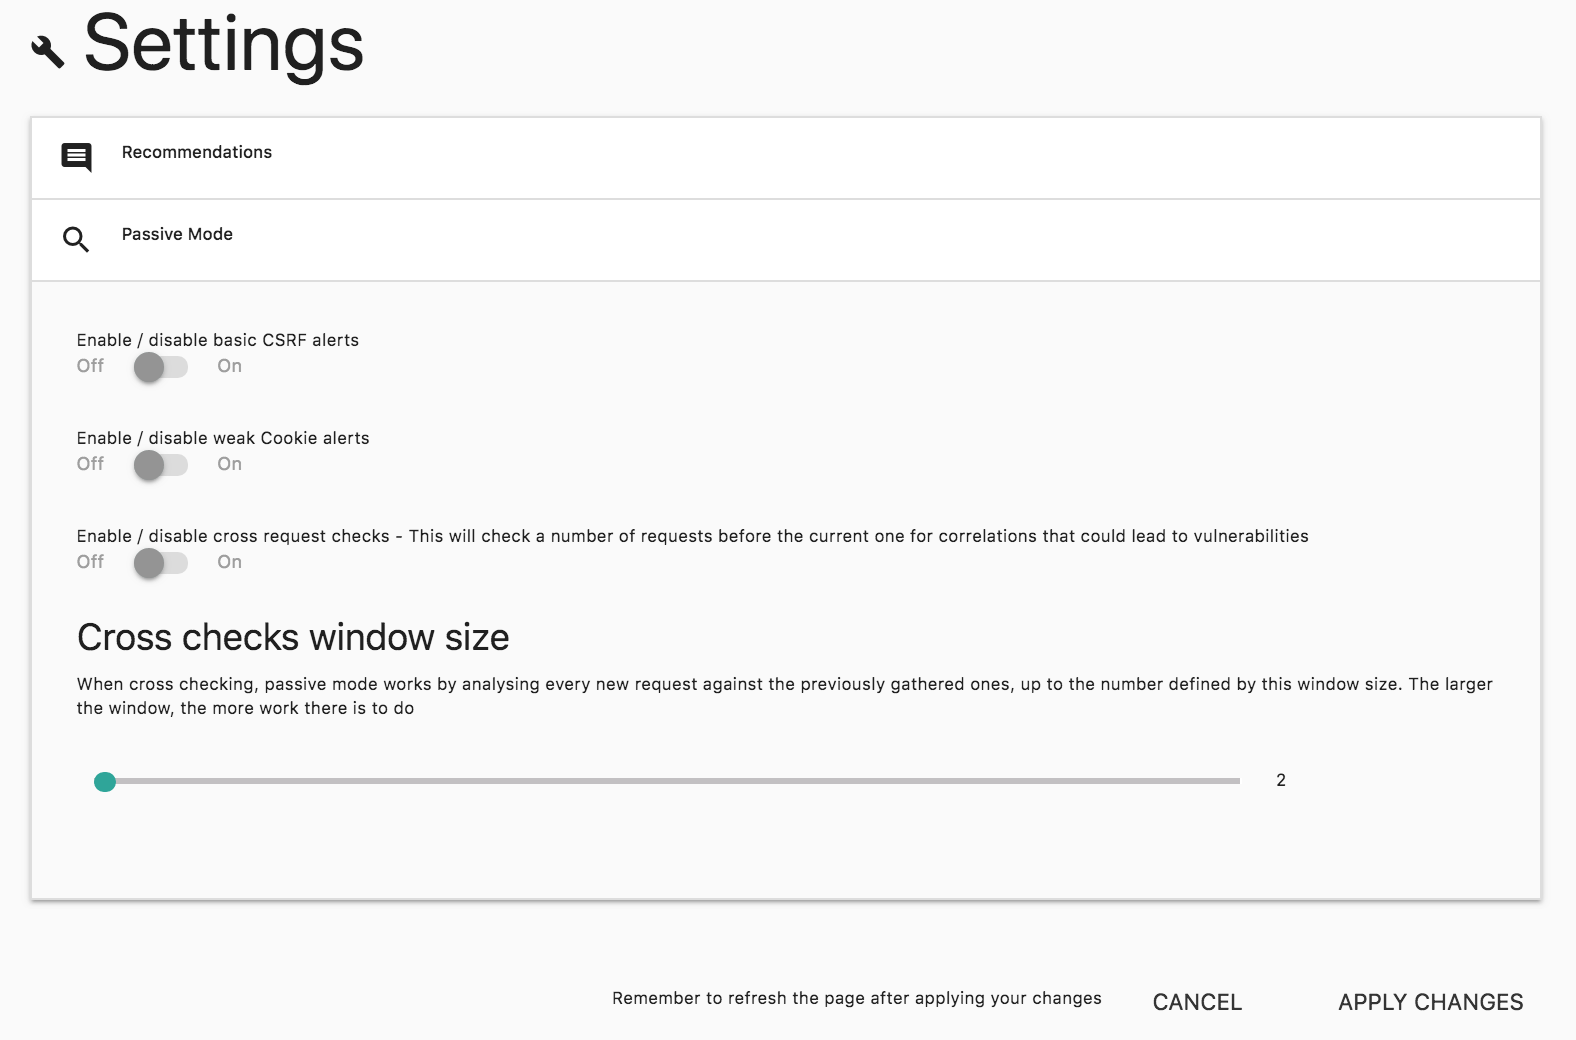
\includegraphics[width=0.9\textwidth]{images/passive_mode_settings.png}
	\caption{The settings tab can be used to configure which submodes are activated within the Passive Mode.}
	\label{fig:passive_mode_settings}
\end{figure}

Once this mode is enabled, any eligible web requests are firstly stored in the \texttt{passiveModeRequests} structure in \texttt{chrome.storage.local}. The analysis is then ran separately per request. The scope of the analysis depends on the activated settings; by default each request is checked for weak security header settings and for potentially dangerous user-controlled inputs that are reflected in responses. The user can also activate further basic CSRF and Cookie safety checks, as well as enabling the \textit{cross checks} feature. 




\subsection{Header Analysis} \label{header_analysis}

This performs some basic checks regarding a set of headers whose presence is designed to improve security in a website. These are:

\begin{itemize}
	\item \textbf{Content-Security-Policy} - This header specifies what sources it trusts content from, in a whitelist manner. XSS attacks abuse the trust that is often (unintentionally) conferred to the source of executable content in a page. With the correct settings, the CSP header will only allow scripts from trusted sources to run. At the same time, since we can specify specific sources as trusted, we can enforce that all content is loaded using SSL by specifying a source with a HTTPS scheme.
	
	\item \textbf{Referrer-Policy} - This policy controls what information to send (if any) on the \texttt{Referer} header\footnote{ Typo intended \cite{refererHeader}}. Many websites use the \texttt{Referer} header to analyse where their traffic comes from, and some even use this to validate permissions to access secure content. However, this may leak sensitive information - this header will usually include the URL of the page which the user was just on. It's often the case that a session ID or other sensitive query parameter is included in the URL, and leaking this information to another website indiscriminately could pose a security risk. The most strict of potential policies here is the \texttt{no-referrer}, which passes forward a blank \texttt{Referer} header. Other, more relaxed alternatives to this policy also exist \cite{referrerPolicy}.
	
	\item \textbf{Strict-Transport-Security} - 	This header (abbreviated to \texttt{HSTS}) allows browsers to determine whether a website should be only accessed using HTTPS or not. There is a small window for a man-in-the-middle attack when using this - if it is the user's first time accessing the website and they access the HTTP version, it is possible for an attacker to hijack their connection and instead connect them to a duplicated site, which allows their credentials to be stolen. Otherwise, as long as the user has visited the safe HTTPS version of the website in question at least once, the \texttt{HSTS} header will have let the browser remember that this website wishes its users to connect to it only through HTTPS, enforcing this for as long as the \texttt{max-age} directive within the header value allows. Additionally, it is recommended that a website also includes the \texttt{includeSubDomains} directive so that any subdomains belonging to this website also enforce a similar policy.
	
	\item \textbf{X-Content-Type-Options} - This header is set to ensure that a defined \texttt{MIME-type} is followed and not changed by a browser. In some cases where the browser is not certain about what content it has just received, it may try to guess this type, which can result in the execution of some (potentially malicious) content. This is called \textit{MIME-type sniffing}, and setting this header to \texttt{nosniff} prevents the browser from doing so.
	
	\item \textbf{X-Frame-Options} - This header can be set to determine whether a website may be rendered in another origin within a \texttt{<frame>}, \texttt{<iframe>} or \texttt{<object>} tag \cite{xFrameOptions}. Denying this behaviour can prevent clickjacking behaviour, where the content from a legitimate website is rendered on a malicious website to trick users into believing they are using the legitimate site.
	
	\item \textbf{X-XSS-Protection} - This is a slightly older header whose behaviour may be made redundant through appropriate use of the \texttt{Content-Security-Policy} header. Nonetheless, setting this header allows the browser to perform basic checks to prevent against reflected XSS attacks, and, depending on the mode set, will sanitize or block the page from being rendered altogether.
	
\end{itemize}

The analysis of these headers does not require that the "recommended" values of these headers are set - although these are \textit{probably} the desired values to be set by the developers, we cannot be sure it isn't intentional on their part to do so. Instead, the extension warns when these headers have not been set, which is a higher indicator of negligence to their importance than a "weaker" setting. If that is the case, an appropriate warning is added to the request in the \texttt{passiveModeWeakHeaderRequests} structure. The \texttt{popup} page will render all the warnings for a request as appropriate. 

\subsection{Reflected Input Checks} \label{reflectedInputChecks}

The process performed here is the same as the analysis part described in the Action Replay section \ref{actionReplay}. A difference between these is that any warnings found in this part will be generated and displayed in the \textit{Passive Analysis} tab in the extension, as opposed to the \textit{XSS} tab.

\subsection{Basic CSRF Checks} \label{csrfChecks}

The principle behind a Cross Site Request Forgery (CSRF) attack is that a website relies on a user's identity to validate actions on their behalf. This identity may be kept as information in the user's browser, perhaps as a session ID stored in a cookie to distinguish this user from other users. The attack results from the user being tricked into performing state-changing actions on the application by an attacker who has exploited the trust mechanism used between the application and the user. These state-changing actions could happen if the attacker has also worked out which URLs the application would fabricate when performing these actions on behalf of the victim. \\

In the context of checking this passively, we employ a very basic algorithm to establish a minimum set of requirements for a page that could be vulnerable to CSRF:

\begin{enumerate}
	\item \textbf{Target pages using client-side authentication} - The most basic means of doing this is to look for a cookie which establishes some means of authentication between the website and the user. The script executing in this part contains a list of well known cookie names known to store this type of information in different web frameworks. This could easily be bypassed by tweaking the name of this cookie slightly (with a number perhaps). Therefore, the check done is whether the cookie in question includes (in any part of its name), the strings contained in the "session cookie name blacklist".
	
	\item \textbf{Focus on pages with content to submit} - The algorithm now searches for any pages that contain a \texttt{form} tag within them. 
	
	\item \textbf{Emit a warning for any which don't contain a hidden input within the form} - One commonly included means of avoiding CSRF by web developers is to add an anti-CSRF token to forms that will be submitted. This adds an element of randomisation to the page, and means that the generated URL when submitting the form will be randomised, making it more difficult for an attacker to consistently generate a working URL that causes users to take undesired actions.
\end{enumerate}

If a page fulfills these checks then it is a potential candidate to a CSRF vulnerability, and the algorithm emits an appropriate warning for this. 

\subsection{Basic Cookie Setting Checks}

When setting a cookie in in the browser, the developer has several directives they can apply to that cookie for the future. When it comes to securing the contents of the cookie, there are 2 key directives a developer can use - setting the cookie to be \texttt{secure} and / or to be \texttt{HttpOnly}. \\

Setting the cookie to be \texttt{secure} means that the cookie will only be set when the request doing so is executed over SSL (that is, using a HTTPS connection). The principle is that cookies may contain sensitive information, so it is not adequate to set or disclose their contents over an unprotected network. The \texttt{HttpOnly} directive is set to prevent access to the contents of the cookie through Javascript's \texttt{document.cookie}, using \texttt{XMLHttpRequest}s or by using the \texttt{Request} API \cite{setCookie}. \\ 

The algorithm here filters out Cookies that are likely to store important information - the list of 'critical' cookies is the same as the one used in \ref{csrfChecks}. If any of these are found, the extension issues a warning for any of these which have been set without the \texttt{secure} and \texttt{HttpOnly} directive. 

\subsection{Request Cross Checks}

The passive mode works by looking at each individual request and its equivalent direct response, and analysing the contents between these two. However, it may be the case that in some vulnerabilities, the weakness is only exposed in a later request/response pair than the initial request which triggered it. This is a close description of \textit{Second Order Attacks} - whether it is a command injection or an XSS vulnerability, these are attacks will only show their effects at a later point than their exploitation. \\

\begin{figure}[h]
	\centering
	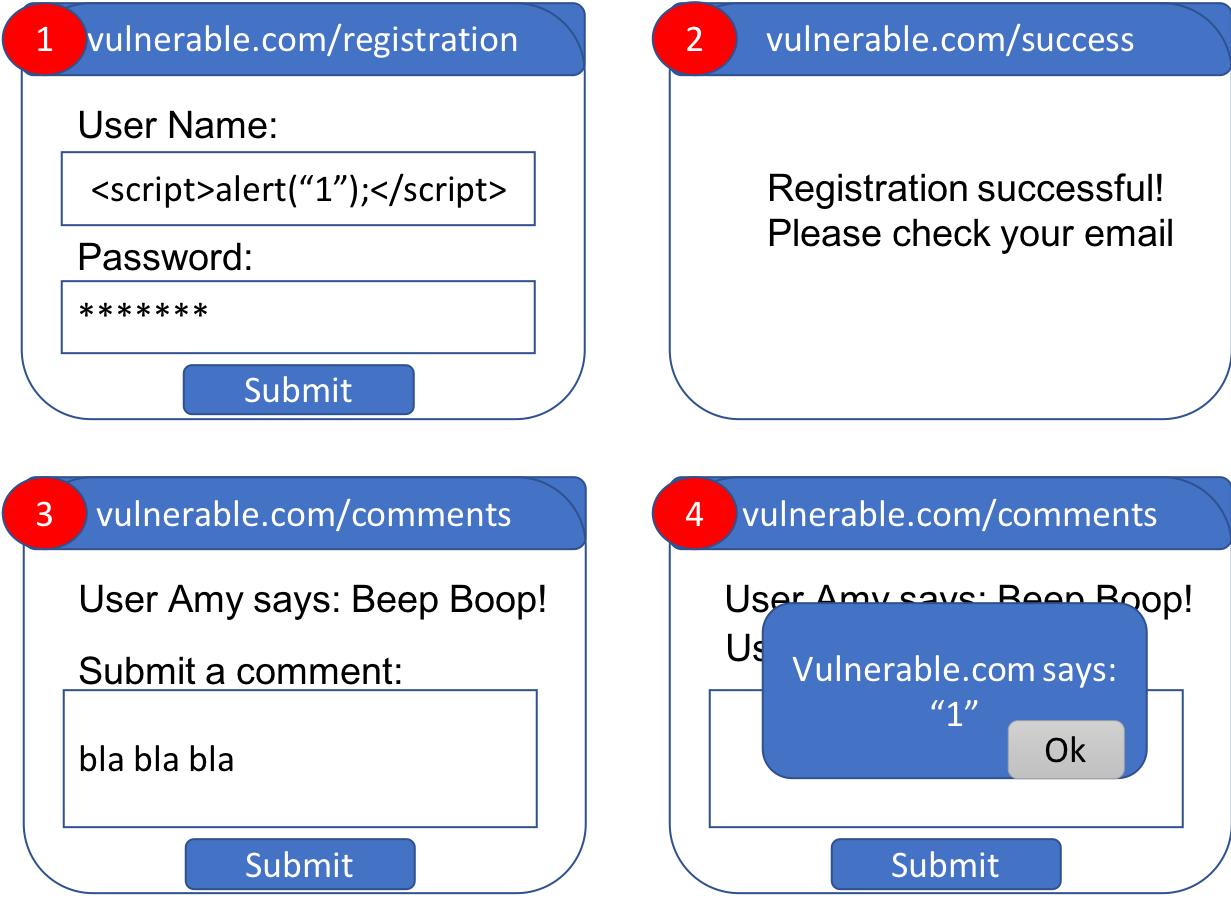
\includegraphics[width=0.8\textwidth]{images/second_order_attack.png}
	\caption{This illustrates a potential second-order XSS attack. In this example, an unsanitized user registration form \textbf{(1)} allows a user to register under a username that could cause a Javascript injection if their username is refelcted elsewhere on the page. There are intermediary steps between this vulnerability and its exploit however - in step \textbf{(2)} we see a registration successful page, and even in step \textbf{(3)} we have not yet experienced the attack. Only in step \textbf{(4)} do we see the effects of the attack as the user name is reflected in the page, injecting and executing the script.}
	\label{fig:secondOrderAttack}
\end{figure}

This mode is our attempt at responding to these types of attacks. Enabling the Cross Checks functionality employs the same algorithm as that used for the \textit{Reflected Input checks} (\ref{reflectedInputChecks}), with the key difference that we are now not only looking at the immediate request inputs that generated the current response, but we also analyse the request inputs of previous requests to check for correlations in the outputs of the current response. Using \ref{fig:secondOrderAttack} as an example, in order to be able to identify the second-order attack, we would need to use a cross-check window size of 4. This is because our latest request \textbf{(4)} is victim to an attack input that was made in request \textbf{(1)}. Hence, setting the cross-check window size to 2 would only additionally look at step \textbf{(3)} in the figure, but this may come up short in terms of identifying such a vulnerability. Naturally, increasing the window size adds more analysis work to be done on every request, and is more likely to find false positives, so it may be difficult to strike a correct balance between not making the window so large so as to clutter the outputs with false positive warnings, but large enough to detect second-order attacks within a web application.

%Mention about 2 different ways of doing it - passive mode with normal cross checks by default - sliding window with eviction of requests.
%Instead I keep window size and cross check only when enabled.

